%%%%%%%%%%%%%%%%%%%%%%%%%%%%%%%%%%%%%%%%%%%%%%%%%%%%%%%%%%%%%%%%%%%%%%%%%%%%%%%%%%
%% Formato de Edición de Artículos a ser publicados 
%% en la Revista Maskana de la Universidad de Cuenca
%% Dirección de Investigación - DIUC
% 
%
%	Versión 1.0, Octubre de 2014
% Ayuda sobre el uso de esta plantilla diríjase a kenneth.palacio@ucuenca.edu.ec
%
%
%%%%%%%%%%%%%%%%%%%%%%%%%%%%%%%%%%%%%%%%%%%%%%%%%%%%%%%%%%%%%%%%%%%%%%%%%%%%%%%%%%%

%Inicio del documento.


% Por favor no modifique el tpo de letra ni utilice otra clase diferente a la indicaca.
\documentclass[11pt]{article}

% Coloque aquí otros paquetes que pueda necesitar siempre que no entren en conflicto
% con los siguientes:
\usepackage{Maskana-template}
\usepackage{graphicx,url}
\usepackage[brazil]{babel}   
\usepackage[utf8]{inputenc}  
\usepackage{multicol}

% UTF-8 encoding is recommended by ShareLaTex     
\sloppy


% Modifique el título del artículo: utilice \\ para dividir en dos líneas.
\title{Platform to promote research in Ecuador using Linked Data and Data mining}

% Edite los nombres de los autores: puede haber varios autores simplemente agréguelos.
% Un autor puede tener varias ailiaciones, sepárelas por coma; tal como se muestra para
% el tercer autor:
\author{Nombre del Primer Autor\inst{1}, Nombre del Segundo Autor\inst{2}, Nombre del Tercer Autor\inst{1,3} }

% Edite a continuación las afiliaciones de los autores:
% Indicando su departamento/unidad/grupo de investigación, universidad/centro/institución
% dirección, ciudad, país y código postal.
% Si varios autores tienen la misma afiliacion, no repita la información. 
% Para ello utilice los índices.
\address{Afiliación del primer autor, nombre de la universidad,\\
  Dirección de la Universidad, ciudad, pais, código postal
\nextinstitute
  Afiliación del segundo autor, nombre de la universidad,\\
  Dirección de la Universidad, ciudad, pais, código postal
\nextinstitute
  Afiliación del tercer autor, nombre de la universidad,\\
  Dirección de la Universidad, ciudad, pais, código postal
  \email{\{primero,segundo\}@universidad.edu, tercero@universidad2.edu}
}

%%%%%%%%%%%%%%%%%%%%%%%%%%%%%%%%%%%%%%%%%%%%%%%%%%%%%%%%%%%%%%%%%%%%%%%%%%%%%%%%%%%%%%%%%%%%%%%%%%%%%%%%%
% Inicio del documento escrito

\begin{document} 

%%%%%%%%%%%%%%%%%%%%%%%%%%%%%%%%%%%%%%%%%%%%%%%%%%%%%%%%%%%%%%%%%%%%%%%%%%%%%%%%%
% En caso que su artículo esté escrito en inglés considere:

%% Note: Use the correct words according to the language of
%% your paper, if you use English:
%Please change ``Referencias'' to ``References''
\renewcommand{\refname}{Referencias}
%Please change ``Tabla'' by ``Table''
\renewcommand{\tablename}{Tabla}
%Please change ``Figura'' by ``Figure''
\renewcommand{\figurename}{Figura}
%Please change ``Agradecimientos'' by ``Acknowledgements''
\acknowName{Agradecimientos}
%%%%%%%%%%%%%%%%%%%%%%%%%%%%%%%%%%%%%%%%%%%%%%%%%%%%%%%%%%%%%%%%%%%%%%%%%%%%%%%%%%%

\maketitle

%Escriba el resumen de su artículo en inglés dentro del siguiente entorno:
\begin{abstract}
(i) mencionar los principales objetivos y el alcance de la investigacion (lo que se hizo, por que se lo hizo y para quien se escribio el articulo?); (ii) describir los metodos empleados en la investigacion; (iii) resumir los resultados obtenidos; y (iv) mencionar las principales conclusiones derivadas de la investigacion. Los resumenes se redactan, por lo general, en tiempo pasado, porque se refiere al trabajo ya efectuado.
\end{abstract}

%Escriba en inglés las palabras clave de su artículo dentro del siguiente entorno:     
\begin{keywords}
English Keywords, \LaTeX{} Template, Revista Maskana, University of Cuenca, DIUC.
\end{keywords}

%%% Escriba las diferentes secciones de su artículo

\section{Introduction}
\label{sec:Intro}

Research in Iberoamerica has increased in recent years. According to the publication of the State of Science 2015 the number of items registered in the Science Citation Index (SCI) [1] grew by 123 \%. Increasing its participation in international databases to increase its local scientific production [2]. One of the most prominent countries is Brazil increased its number of publications by 2.5. However, it has several limitations, as the amount of resources invested in research in contrast to the world average. should be noted that in Latin America is the second fastest growing in the world after Asia [3]. It has a wide range of areas of knowledge, in addition, each country has different strategic ways to address the problems of a region. Which provides a set of solutions that can be an advantage compared to first world countries in the field of research, as these solutions should be able to cope with this heterogeneity in Latin America. 


One focus of the IHE  (Institutions of Higher Education) of Latin America is to contribute to the sustainable development of society through the cooperation of students and teachers, driven or promoted  by research. Currently, certain information about researchers and their bibliographic resources are scattered among various digital repositories or bibliographic databases. When you need to propose projects with several researchers in a specific area belonging to different IHE  , raises questions such as: Who works in similar lines of research? or how you can create a network of researchers in a common area when we do not know if they exist? In addition, research to define the profile of a person in analysis, get your articles, in that magazines that were accepted, among others, need to access multiple data sources. Given that this process is manual, syntactic and different for each source of bibliographic resources available on the Web.

Expand the scope of this knowledge base will allow the entire Ecuador to have a centralized digital repository which has information of Ecuadorian researchers based in bibliographic resources. This project aims to encourage interagency collaboration and obtain as a result of this work a validated semantic repository, locate researchers working in similar research areas and provide updated information accessible and reusable. Enhancing the generation of research networks with academic peers in the region and provide greater opportunities for cooperation and collaboration to the participating institutions.


Different works have been accomplished like: 
Semantic Scholar
GeoLink
Es necesario contar con herramientas que faciliten el trabajo a los investigadores, en el que varios proyectos han trabajado, como: Semantic Scholar[4] y [5]. Sin embargo estas herramientas abarcan un dominio limitado, es decir, son herramientas que tratan publicaciones y autores locales o de una determinada area de conocimiento como por ejemplo informatica.  La estabilidad de las herramientas que traten este problema es fundamental ya que cada dia surgen nuevos aportes cientificos, nuevas areas de estudio, y cientos de investigadores se suman en proyectos tanto locales, como internacionales y multidisciplinario.  

This document presents a platform developed to detect similar areas of knowledge between  researchers and build interagency working groups. Using semantic integration of bibliographic databases available on the Internet like: Google Scholar, Microsoft Academics, Digital Bibliography \& Library Project (DBLP), Scopus and Knowledge Discovery in Databases (KDD). The rest of this paper is organized in the following way: section II presents some theatrical foundations used. The process for extraction and integration from bibliographical databases is described in section III and section IV the presents how we applied clustering to find similar areas and build research networks. 


\section{Theory}
\subsection{Bibliographical Ontologies.}
The Bibliographic Ontology (BIBO) \cite{bibo} developed by Fr\'ed\'erick Giasson and Bruce D’Arcus describe bibliographic things on the semantic Web in RDF. This ontology can be used as a citation ontology, as a document classification ontology, or simply as a way to describe any kind of document in RDF. It has been used to describe publications, citations, conferences, etc. This ontology also helps us to define a common data model for authors and publications on the platform, but it's not enough because we have publications with special properties that don't be in BIBO, so it is necessary to extend this ontology so that our data fits. 

An ontology that its similar to BIBO is  FaBio the FRBR-aligned \cite{o2011frbr} Bibliographic Ontology that is bears many similarities with BIBO, including its overall scope and intention, and the inclusion of PRISM and DC Terms data properties.  this ontology is structured according to the FRBR[*] conceptual model, in which publication entities are described from four different and correlated points of view, those of Work, Expression, Manifestation and Item, each of which is a FRBR Endeavour. FaBiO was developed to describe anything a research scientist might need to reference.

selected ontology to describe the bibliographical resources in the plaform is BIBO because it offers the advantages as semantic reasoning support of an OWL 2 DL, simplicity, expressiveness agil which are not clearly defined in the ontology Fabius. support to make inferences about the data is important if what we do is finding information. Furthermore Fabio offers features to mix with other ontologies which is not necessary in the project at this early stage.
\subsection{Apache Marmotta Platform.}
Apache Marmotta provide an open implementation of a Linked Data Platform that can be used, extended and deployed easily by organizations who want to publish Linked Data or build custom applications on Linked Data[]. This platform have a recommendation that is being developed by W3C. Among the main features we can mention read-write Linked Data, RDF triple store with transactions, versioning and rule-base reasoning, SPARQL and LDPath query languages, transparent linked data caching, integrated security mechanisms. In December 2013, it has been nominated as \emph{one of the ASF's most active projects}[]
Apache Marmotta comprises  some components but specifically has been used JavaEE web application providing the Linked Data server, KiWi a Sesame-based triple store built on top of a relational database and  LDClient, a client that allows retrieval of remote legacy resources not available as Linked Data. Through the library Linked client data can consume data from publications from bibliographic databases and whether they are described with some ontologies, or otherwise they are described using ontology BIBO.



\subsection{Text clustering}

Document or Text Clustering [6] is a subgroup of the data clustering field [5] which is an unsupervised learning process. Clustering consists in organize items from a collection into groups of similar items, where each group is called cluster. Each cluster have a set of similar items to each other -  generally based in a measure of similarity - but dissimilar to other items that belongs to other clusters. Clustering should not be confused with classification, because documents does not have a class assigned. Documents in text clustering are represented as a bag of words, which give a problem of high dimensional spaces. [1] There is no way to know the number of clusters, size or shape before to apply clustering. A human or an algorithm are who determine these parameters. [2,3].

Clustering is not as simple as it seems, to do more than just grouping, we could produce a disjoint (exclusive clustering) or overlapping partitions. Clustering algorithms could be divided in two flavours, discriminative and generative types. Discriminative algorithms are based on a distance metric to find a similarity between documents. While, generative algorithms the model is squeezed to fit in the distribution to produce cluster centroids. Finally clustering has been used in many areas like information retrieval [7], outlier detection [4], to improve queries returned by search engines [7], etc. 

\subsection{K-Means}

K-means is a simple and old algorithm for clustering [8]. It was proposed by Stuard Lloyd [9] and it is still been used in many fields of science. The user should determine the number of cluster k, which could be set based on the dataset and the number of clusters you need. It is a rude way to estimate the number of clusters, but it is a useful point to start doing experiments. The distance measure that you use in K-means it is vital to determine the quality of the clustering process. 

K-means is complex when it is executed with very large data sets the memory of a single computer could not be enough [10]. The K-means algorithm will do the following steps:
\begin{enumerate}
	\item Determine the number of clusters k
	\item Initialize the the centroid or center of these clusters.
	\item Determine the distance of each point to the centroids and assign the point to this cluster.
	\item Determine the centroid coordinate
	\item Stop when there no new reassignments or have reached the maximum number of iterations. 
\end{enumerate} 

\subsection{Latent Dirichlet Allocation}

Latent Dirichlet Allocation (LDA)\footnote{Apache Mahout implements Collapsed Variational Bayes (CVB) algorithm for LDA [12]} [11] is a generative algorithm to cluster words into topics. LDA assume that the whole corpus has k number of topics and each document is about these k topics. Then a document could have a mixture of topics with different probabilities. LDA explained as an analogy is when a person read a document has certain topics in mind. 

Usually a topic is a word from a pool of words that belong to a document. LDA has been successfully applied for tag recommendation[13], find scientific topics [14], web spam clustering[15], etc.

\section{Consolidate Data}


Scientific publications of Ecuadorian authors are available in different bibliographics databases on internet at each source varies the information on scientific activity of an author. For example Scopus sources  save affiliation of authors, tables, graphs of publications, authors study areas, etc. DBLP features does not cover. For this reason is necessary make a unification of these bibliographic resources with different disciplines, structures with features that feed a common data model. For this task has been defined as the first phase the extraction of scientific publications from different external bibliographics sources, after a data integration process and disambiguation of authors and their publications , and as a third phase defined a method to  data update add information to allow a controlled way, facilitating access, discovery and reuse of scientific resources.
The development of the first stage of the platform faces two challenges. 1) Extracting data from heterogeneous bibliographic sources. 2) Integration of publications with different data formats, vocabularies and conceptualizations using ontologies and vocabularies to describe bibliographic data in a single model.

\subsection{Extraction data of bibliographic databases}
The extraction process of publications is responsible for obtaining information from scientific articles Ecuadorian authors from various external bibliographic databases previously analyzed as Google Scholar, Microsoft Academics, Scopus, etc. Each of these data sources operate in a different way, so the extraction service adapts to each of the data sources. For the extraction of publications should be considered that the data source consisting of an API access, because if data collection is not available through an API the data quality is poor as demonstrated below. The collection of scientific publications is the first phase that will allow us to obtain data which depend on the following phases, because if the data are erroneous alter the expected results.

\subsubsection{Analyse of access on bibliographic resources.}
Google Scholar, Scopus, DBLP, Microsoft Academics, Semantic Scholar, GeoLink, etc made available tools that facilitate scientific research. They differ in the form and manner that publish these resources, and the respective policies of each resource or bibliographic database. In some cases it has access to the abstract, references, citations or full article in PDF format and in other cases only the metadata has given publication. As for this platform is considered to use different sources in order to account for the heterogeneity of the sources.
Certain data sources have API access to information, but when a source does not have this access can be a problem. The tools that extract should be adapted to the context in which these resources for example websites, sets of documents in pdf format or any type of bibliographic information which is not available through an interface with certain characteristics such as compatibility are published and reliability. If not considered sources like Google Scholar that does not have an access interface information to be analyzed may be limited. Therefore the extraction service adapts to the source in the event that this does not consist of an API, however data from it will not have the same quality as data that come from a source consisting of an API access.

For the development of the first prototype of the project has been selected four bibliographical databases such as Microsoft Academics, Google Scholar, Scopus, DBLP  to cover different types of databases and present a scenario in which the main problems involved in making the extraction and integration of bibliographic sources. Subsequently, the platform should allow seamlessly add new data sources and this process should not affect the platform operation.

\subsubsection{Analysis of the data models of bibliographic resources data source.}

The different bibliographic databases provide their own resources with a logical structure which makes the data model for each source is different despite dealing with the same type of information. Bibliographic resources are not 
ruled by a standard or comprehensive model encompassing all properties as authors, appointments, conferences, knowledge areas, etc. in the same way. Some features such as DOI, ISBN, format bibliographic references of resources are ruled by International Standard Bibliographic Description (ISBD), ISO 690, etc. However it is not enough if we need a common data model to facilitate the processing of scientific publications.

In Figure [1] you can see the data model between two bibliographic databases: Microsoft Academics and Springer Open Access API API that represent the diversity of models of data between bibliographic databases. This heterogeneity of models represents the challenge of integrating various sources, taking into account that some sources don't publish your data model. Therefore before adding a new data source to the platform must perform an analysis of its structure with respect to models already being used for the purpose of assigning correspondences between model features the new source and model common data.
 \begin{figure}[ht!]
	\centering
		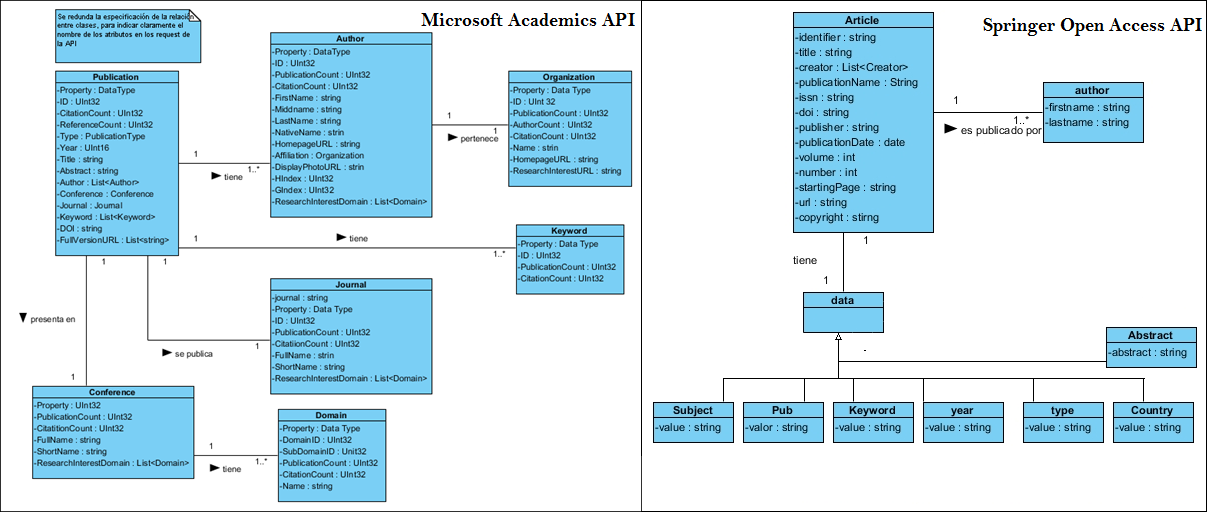
\includegraphics[height=5.2cm]{modelosMA_Springer.png}
	\caption{Data Models of Microsoft Academics API and Springer Open Access API.}
	\label{fig:Escudo2}
\end{figure}

\subsubsection{Architecture extraction service publications.}

The architecture for service publications extraction is implemented generically adapted to the source. In Figure * you can see the architecture of extraction service , which have exposed the different data sources to be consulted, which some of them have API access to data. The module requests the service publications extraction publications of an author sending as parameters the author names. The service searches all bibliographical sources external publications of the author and if this are not described in any ontology then describes using BIBO. Finally these data recorded in RDF are sent publications module, then be processed to a central repository.



\subsection{integration of authors an publications}

The integration process is responsible of unify the publications of all bibliographic sources. The extraction service keeps publications in a respective graph for each source, and it has a graph of publications DBLP, Scopus, etc. Integration service unifies all graphs either publications or authors in a central graph called wkhuska. For this unification we find characteristics between publications and authors in the platform. the origin of the publication is also stored and whether a publication is similar to another is as described with  SameAs  property, and equally form  the authors, this descriptions are used to disambiguate publications by the same author. As a result the unified data integration process are obtained and available through Apache available marmot SPARQL.
 

In view of the diversity of data models bibliographical sources a common data model which encompasses the main features of each source publications was raised. The model proposed is described using ontology BIBO (bibliographic ontology), which is an ontology is used to describe bibliographic entities as books, magazines, etc. [10]. This ontology is used to describe bibliographic resources and are listed in RDF. The authors are described using ontology FOAF (Friend of a Friend), it is an ontology used to describe people, their activities and their relationships with other people and objects. The common data model is presented in Figure [2], wherein the different attributes and relationships necessary for the representation of library resources in the platform.

 \begin{figure}[ht!]
	\centering
		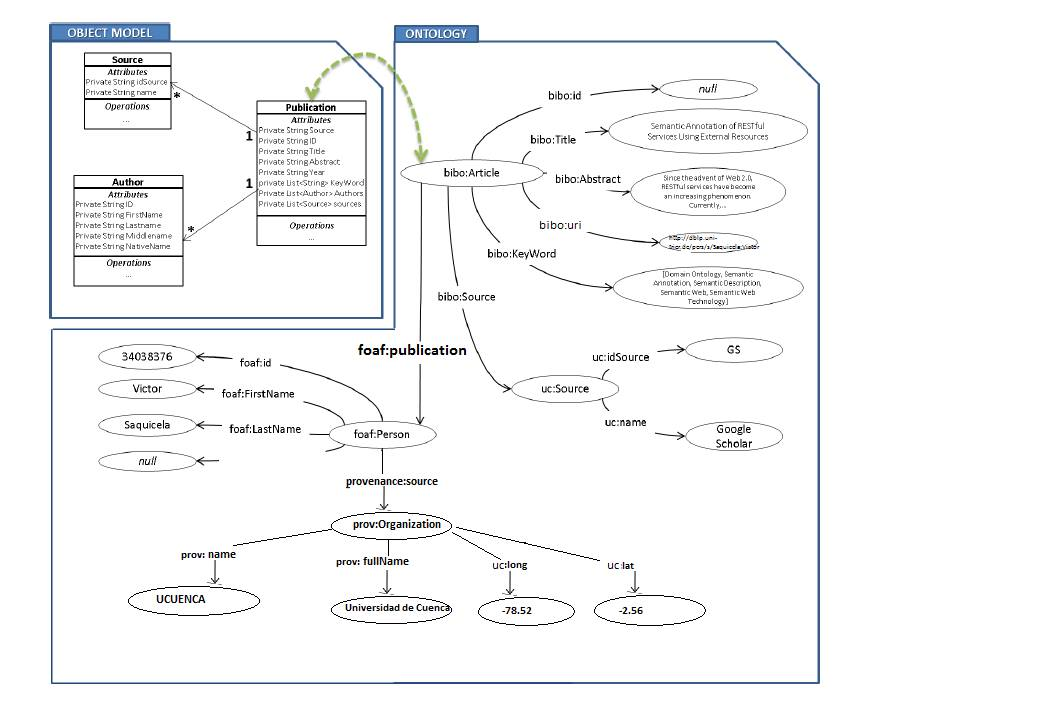
\includegraphics[height=8.2cm]{dataModelCommon.png}
	\caption{Common data model publications.}
	\label{fig:Escudo2}
\end{figure}
 
The incompatibility between different data models bibliographical databases is handled through a process of mapping, so that a correspondence between the properties of the attributes of publications and bibliographic source model proposed common data set. This process is necessary to specify the time manually correspondences between the properties of publications and model. When adding a new source is must identify the correspondences between data models. However, this process should be done automatically taking into account that this is a defined domain and similar ontologies.
There are studies which perform making an automatic annotation of web services REST, analysing their input and output  on a bus service \cite{ortiz}, it would be useful in our case for access to API services and add bibliographic databases in a way easier and faster thus enriching our repository.

It has been necessary to have materialized data authors and publications with the aim of finding correspondences between these locally since the other option is to recover the publications at the time they are needed ie make a request for this to the source in a given moment. The time between making a request to an external source and the mapping takes an average of twenty seconds. So the fact is justified d realize the offerer high availability and speed bibliographic resources to consult the publications of a specific author.

\subsection{Disambiguation of authors and bibliographic resources.}

The platform have publications from different sources by the same author and to perform this task has several entities of the same person possibly with the same publications, so it is necessary to discover that these authors are the same entity. The prototype developed allows you to define a single record of an author in a central graph based on various entities of the same author of different publications providers. The procedure was performed for this purpose is to analyze the publications of authors who are theoretically the same person with the same publications, unifying them based on a priority set based on experiments. For example the most reliable source is the service Scopus, because other sources of data are inconsistencies when search as the next author   \textit{Juan Pablo Carvallo Vega} and \textit{Juan Pablo Carvallo Ochoa} if we make this search possible that certain data sources provide us the same publications although locally in our repository are two different people. With the method implemented this problem however is necessary to feed this method more rigorous techniques with the aim of identifying a more concrete form to the authors and their publications present in the platform is. Arvin Varadharajalu and Wei Liu1 \cite{varadharajalu2011author} have an algorithm to disambiguation using the affiliation, email, Url, Organization, Co-Authors, etc. Making in context disambiguate authors and publications, so it is necessary to have more information about the author validated to feed disambiguation algorithms on the platform.

In Figure [3] you can see the diagram of the method implemented for disambiguation of authors and publications. As the first step is loaded into memory publications specific chart such as the graph DBLP or Microsoft Academics, etc. each publication is processed asking if first is already in the repository, if not all the properties of the publication as well as the other publications of the author of the publication being processed at that time we will call P1 is removed. It is also extracted from the central graph in the event of any publication the author of P1 and a comparison between the publications of the graph of the supplier and the publications of the Central graph, if matches between these publications is established is made that the author is already present in the central graph and publication P1 is added to this author. In the event that the author's publications P1 are not in the central graph states that it is the first record of the author and their publications. This process assigns a single central author different resources by the same author repeated in each graph provider publications.



\begin{figure}[ht!]
	\centering
		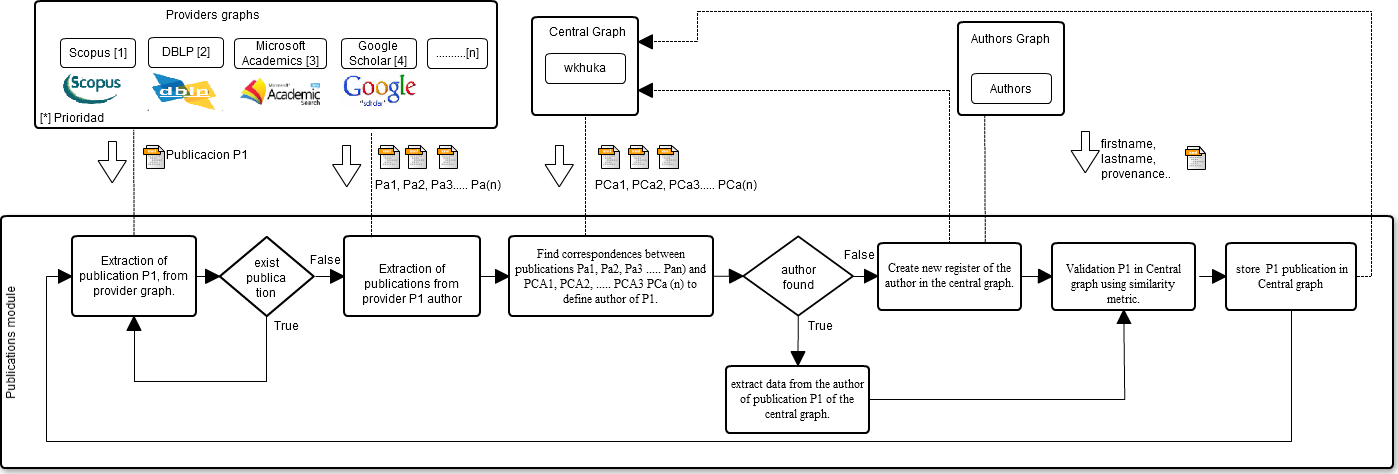
\includegraphics[height=5.2cm]{desambiguationProcess.png}
	\caption{Disambiguation Process.}
	\label{fig:Escudo2}
\end{figure}

\subsection{Analysis and implementation of data update methods.}

Bibliographic  resources must be updated at a frequency set according to the number of authors, literature sources, repositories Ecuatorianos authors, etc. The frequency with which a new library resources published author is unknown which is considered an update of information by set of authors. For example it is possible to perform an update of scientific publications of all authors of the University of Cuenca getting their new publications. It is defined methods therefore incremental update not an update of the repository which would take a long time defined by the number of authors being necessary.
The process begins with a selection of a set of authors to update what the authors repository available to each higher education institution such as University of Cuenca (UCUENCA). Army Polytechnic School (ESPE), etc. This process is done with expert intervention activating the selected source manual. Once the set of selected authors to update, the data required for the update is loaded in memory respective scientific publications in a bibliographic database as defined by the expert may be Scopus, DBLP, etc. If changes are published by the authors information is added to the platform.
  
The number of records of authors on the platform are around ninety-seven thousand so based on experiments when extraction publications all registered authors processing time is too long that can be in is done order of weeks and if a fault occurs in this process should start from scratch. The method implemented timely update has control over the source of publications to use, because such sources as Scopus for example allows a certain value share requests and if this value is exceeded the API blocks access to its resources.

 
Because they do not have relevant information to more than names and surnames of the authors, it is a difficult task to differentiate between two authors with similar names, so that the process presented presents difficulties arise names like \textit{Mauricio Espinoza Mejia} and \textit{Mauricio Espinoza Ana} is a need for more information from the authors to find a relationship between authors and their publications. As a next step in this process is extracting the keyword from registered authors in the source, so that a more concrete relationship between these keywords and the publications of Ecuadorian authors find jobs.
The data still contain erroneous information is not yet due to insufficient data with which to disambiguate authors according to their field of study. For example you can consider using keywords of the work done by the authors in order to identify whether the publications obtained by the service relate to the keywords of local works of the author.


\section{Detect Similar Areas}


In this section, we outline the web service built for data processing . The service has been called KODAR that means "Discovery Of Knowledge Research Areas" with the words a little bit jumbled. It uses Apache Mahout to execute algorithms of machine learning. We choose mahout for the ability to deal with massive datasets, it is a scalable Java library and we could profit of the distributed computation, because It is built upon Apache Hadoop. KODAR has three main stages that are: Discover similar areas, detect researchers networks and find a general topic area. The whole implementation is open sourced and available on our GitHub repository.


\subsection{Discover similar areas}

Broadly, keywords of academic literature talk about a certain topic area or methodology. Detecting similar areas based in the keywords . It could help us to detect researchers with interests in common and open up an opportunity to generate new research projects. Boosting interagency collaborative work and form cooperative research groups.

Firstly, we disjoin our data, because we just need to process the keywords to detect similar areas. Other fields like author or title of the publication are stored in a separate file. Both files are converted in a specific Hadoop file format that is SequenceFile\footnote{Mahout also use Sequence files to manage input and outputs of MapReduce and store temporary files.}. This file stores key/value pairs, where the key is a unique identifier and a bunch of keyword that belong to a paper are stored as a value. Same happens in the another file with the difference in the value pair. We store the remaining fields.

It is necessary to do some procedures before to clustering the data into Mahout. Data has been preprocessed to convert text in numerical values, but not all the keywords have the same relevance. The weighting technique used to magnify the most important words is Term frequency-inverse document frequency (TF-IDF). The weighted values are used to generate the Vector Space Model (VSM) where words are dimensions. The problem with this VSM generated is that words are entirely independent each other and It is not always true. Sometimes words have some kind of dependency like Semantic with Web. In order to achieve this dependency we use collocations. At the time of writing, we are executing our experiment using bi-grams and an Euclidean norm (2-norm), which can change. In future experiments, It will be interesting to generate vectors using Latent Semantic Indexing (LSI) or apply a log-likelihood to take words that mostly have the chance to go together. So in the long run, we have our vectors completed to clustering.

We start with the vectors generated to execute K-Means algorithm in Mahout. It was executed using a Cosine distance measure as the similarity measure. RandomSeedGenerator\footnote{it is used to generate random centroids} was used to seed the initial centroids. The experiment were set to 100 maximum of interactions and the value of k varies according to the number of data extracted from the different bibliographic databases. Once the algorithm finishes we have our similar areas based in a bunch of keywords.


\subsection{Detect researchers networks}

We have discovered similar areas, now it is time to detect what researchers could be interested to work together based in the ares they are working on. We have developed a MapReduce model to accomplish it as you can observe in the figure \ref{fig:Escudo2}. First, we sorted the name of clusters accord to the unique identifier generated and merged each cluster with their original keyword (before to preprocess). In our final job, we merge the resulting file of the first stage (Sort \& Join) and the additional file containing the remaining fields (title, author) from KODAR?s first stage. Finally, we get a file with all the original fields, plus a field showing the cluster that a row belongs.

\begin{figure}[ht!]
	\centering
		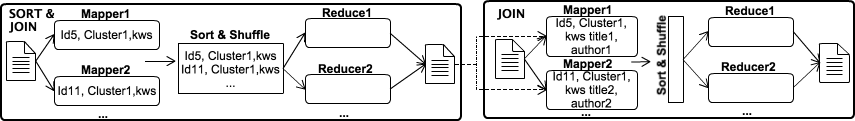
\includegraphics[height=2.2cm]{findka.png}
	\caption{MapReduce model}
	\label{fig:Escudo2}
\end{figure}

\subsection{Find a general topic area}

Our search engine could increase performance in searches by finding a general topic area based in the words that belongs to a cluster. We can respond to specific queries (i.e.: show all researchers working in a specific area or all subareas belonging to a general topic area).

We use WordNet\footnote{it is a lexical database for the English language that is used for text analysis applications.} \cite{FellbaumB98}  \cite{smith:99} \cite{wordnet:01} to find synonyms, hypernyms, hyponyms and the concept of a word for all keywords in a cluster. It helps to find a common meaning in the way that words could occur together and find similar meanings. In other words, with the group of word set up we could find a concept or a topic for each cluster.

We applied Collapsed Variational Bayes (CVB) algorithm that is an implementation for Latent Dirichlet analysis (LDA) in Mahout. We use all the words generated by WordNet plus the title and keywords of each publication to find a broader topic based in multiple subtopics described by the keywords. We use Mahout RowId to convert Term Frequency (TF) vectors into a matrix. The CVB algorithm was executed with the following parameters: 1 for the number of latent topics and 20 maximum interactions. This job is applied to each cluster.

Finally the results of three KODAR?s stages are exported in different formats, but one of most import is the Resource Description Framework (RDF) file. Figure \ref{fig:Escudo2} shows the concepts and relationships used to export the results. The full arrow symbolize a relationship between classes and the dash arrow symbolize a common relationship.

\begin{figure}[ht!]
	\centering
		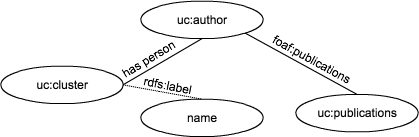
\includegraphics[height=2.2cm]{anotacion.png}
	\caption{MapReduce model}
	\label{fig:Escudo2}
\end{figure}

\section{Results}



We are going to show the interpretation of a taken sample cluster  as result\footnote{All results can be analyzed on the web platform: \url{http://investiguemosjuntos.cedia.org.ec}}. We find that all the words listed below belongs to the general topic area of physics. Researchers that are working in the areas listed of physics are Fern\'andez Tapia, Jaime E, Torres Arteaga, Christian Alejandro and Aguilar Romero, Gino.At last, a research project could be proposed with people that are working in similar areas. 

\begin{multicols}{2}
    \begin{itemize}
	\item Inelastic Scattering
	\item Flow Measurement
	\item High Energy
	\item Fourier Coefficient
	\item Bose Einstein Correlations
	\item Monte Carlo
	\item Three Dimensional
	\item Center of Mass
	\item Large Hadron Collider
	\item Charged Particles
	\item Correlation Function
	\item Proton Proton
	\item Particle Physics
	\item Experience Repor
	\item Elliptic Flow
	\item Heavy Ion Collision
	\item Particle Production
	\item Particle Emission
    \end{itemize}
    \end{multicols}
    



\section{Conclusion and Further Work}

Lo esencial de esta sección es un resumen de las conclusiones importantes y de sus 
implicaciones en el área de investigación sobre la que trata el artículo. Tradicionalmente, las 
conclusiones ofrecen una descripción (resumida) de los objetivos principales del marco teórico, del 
rigor metodológico, de los resultados, el uso e impacto de los resultados, la originalidad y el tipo de 
contribución, y de los desarrollos futuros. \cite{knuth:84}, \cite{boulic:91} y \cite{smith:99}. Para mayor información sobre el formato de las referencias diríjase al enlace:\\ \url{http://diuc.ucuenca.edu.ec/revista-maskana?download=17:guia-autores-maskana}


In the process of extraction of scientific publications we use only the names of the author, for searches of publications, which generates erroneous information for example people with the same name but that  do not work on the same subject. The solution for this problem  is proposed as future work to establish a better partnership between publications and authors, so you can discern whether a publication is linked to the research of a particular author, in otherwise discard this data, improving the quality of information platform.


%%%%%%%%%%%%%%%%%%%%%%%%%%%%%%%%%%%%%%%%%%%%%%%%%%%%
%% Sección de Agradecimientos / Reconocimientos
%% Opcional - Se puede eliminar por completo en caso
%% que su artículo no requiera de la misma.

\begin{acknowledgements} 
  En esta sección se agradece de manera cortés por la ayuda: científica, de redacción y 
técnica (equipo y otros materiales especiales) recibida de cualquier persona o institución. Además, en 
esta sección se expresa también un reconocimiento por la ayuda financiera externa (como 
subvenciones, contratos o becas) recibida tanto para la realización de la investigación como para la 
preparación del artículo. Debe ser breve.
\end{acknowledgements}



\bibliographystyle{MaskanaStyle}
\bibliography{MaskanaBIB}

\end{document}
